En esta secci\'on se analiza cada \'indice. Morbi accumsan nec est ut malesuada. Donec metus augue, commodo eget leo et, sodales vulputate libero. Donec eu sollicitudin ligula. Quisque tempor, tellus ultricies vestibulum suscipit, leo dui porta lectus, sed viverra quam est vitae nunc. In vehicula risus ac nibh tempor vehicula. Donec ut finibus nisi, non ullamcorper neque. Vivamus eget viverra metus. Sed hendrerit ipsum porta tellus condimentum facilisis. Nulla eros neque, commodo at tincidunt vitae, fringilla nec nunc. Pellentesque eleifend suscipit ipsum vitae efficitur. Aenean at sem et mi ultrices faucibus en la Tabla \ref{stats}.


% Table created by stargazer v.5.2.2 by Marek Hlavac, Harvard University. E-mail: hlavac at fas.harvard.edu
% Date and time: jue., jul. 05, 2018 - 3:51:19 p.m.
\begin{table}[!htbp] \centering 
  \caption{Medidas estadisticas de los datos} 
  \label{stats} 
\begin{tabular}{@{\extracolsep{5pt}}lccccc} 
\\[-1.8ex]\hline 
\hline \\[-1.8ex] 
Statistic & \multicolumn{1}{c}{N} & \multicolumn{1}{c}{Mean} & \multicolumn{1}{c}{Median} & \multicolumn{1}{c}{Min} & \multicolumn{1}{c}{Max} \\ 
\hline \\[-1.8ex] 
IDH & 32 & 0.802 & 0.804 & 0.691 & 0.879 \\ 
Poblacion.Cabecera & 32 & 1,196,730.000 & 717,197 & 13,090 & 10,070,801 \\ 
Poblacion.Resto & 32 & 360,590.300 & 268,111.5 & 21,926 & 1,428,858 \\ 
Poblacion.Total & 32 & 1,557,320.000 & 1,028,429 & 43,446 & 10,985,285 \\ 
\hline \\[-1.8ex] 
\end{tabular} 
\end{table} A continuaci\'on se muestra el histograma para el \'indice de desarrollo humano en Colombia. (Ver figura \ref{barplot1})
\begin{figure}[h]
\centering
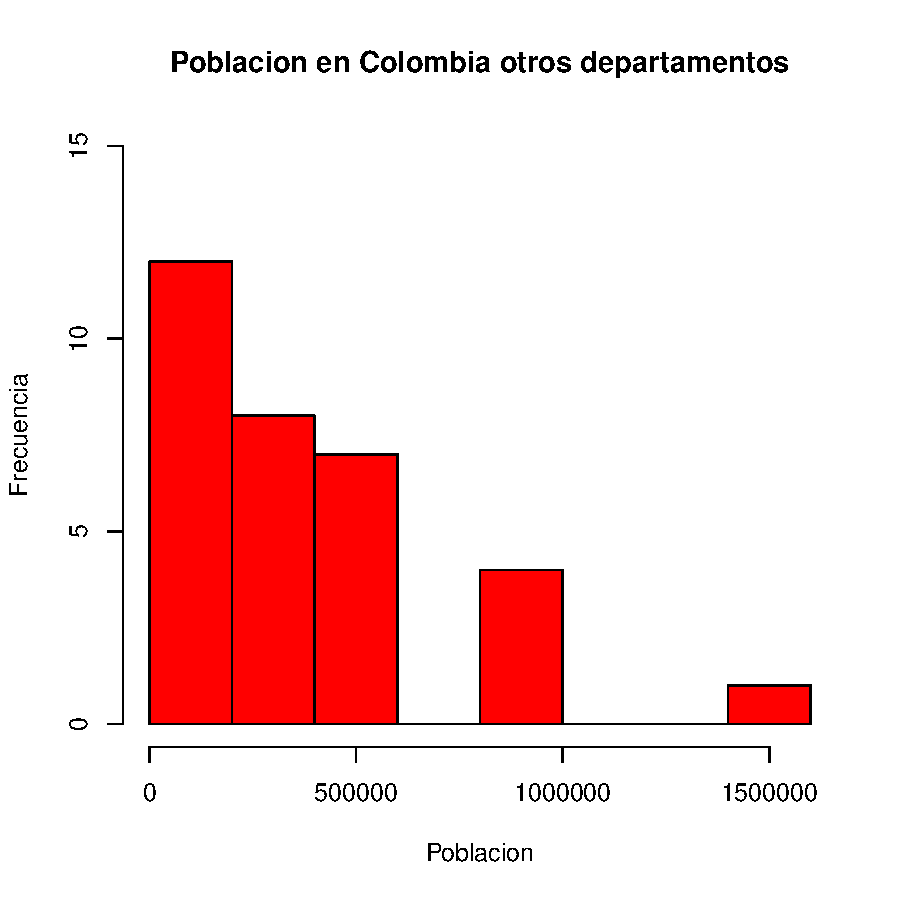
\includegraphics{univariada-summaryDatos}
\caption{Histograma del IDH en Colombia para los 32 departamentos}
\label{barplot1}
\end{figure}

En la figura \ref{barplot2} se muestra el histograma para la cantidad de habitantes en los departamentos de cabecera, mientras que en la figura \ref{barplot3} se muestra la poblaci\'on para el resto de departamentos.
 
\begin{figure}[h]
\centering
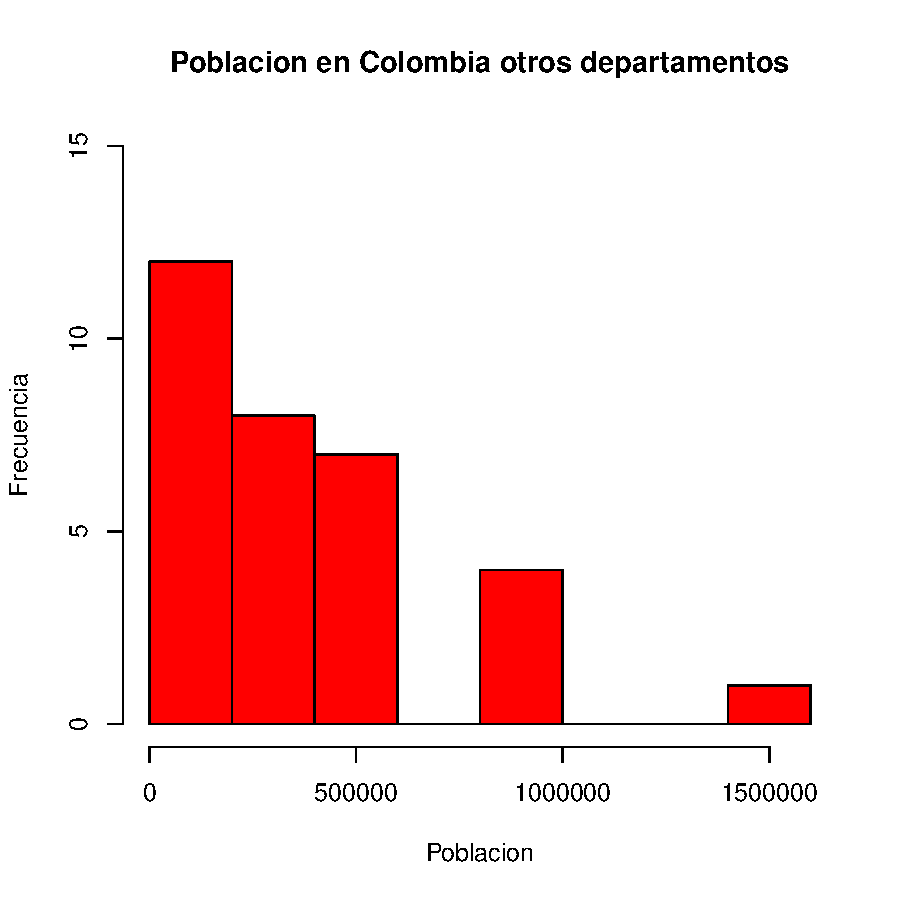
\includegraphics{univariada-summaryDatos}
\caption{Histograma de la poblacion en Colombia para los departamentos de cabecera}
\label{barplot2}
\end{figure}
\begin{figure}[h]
\centering
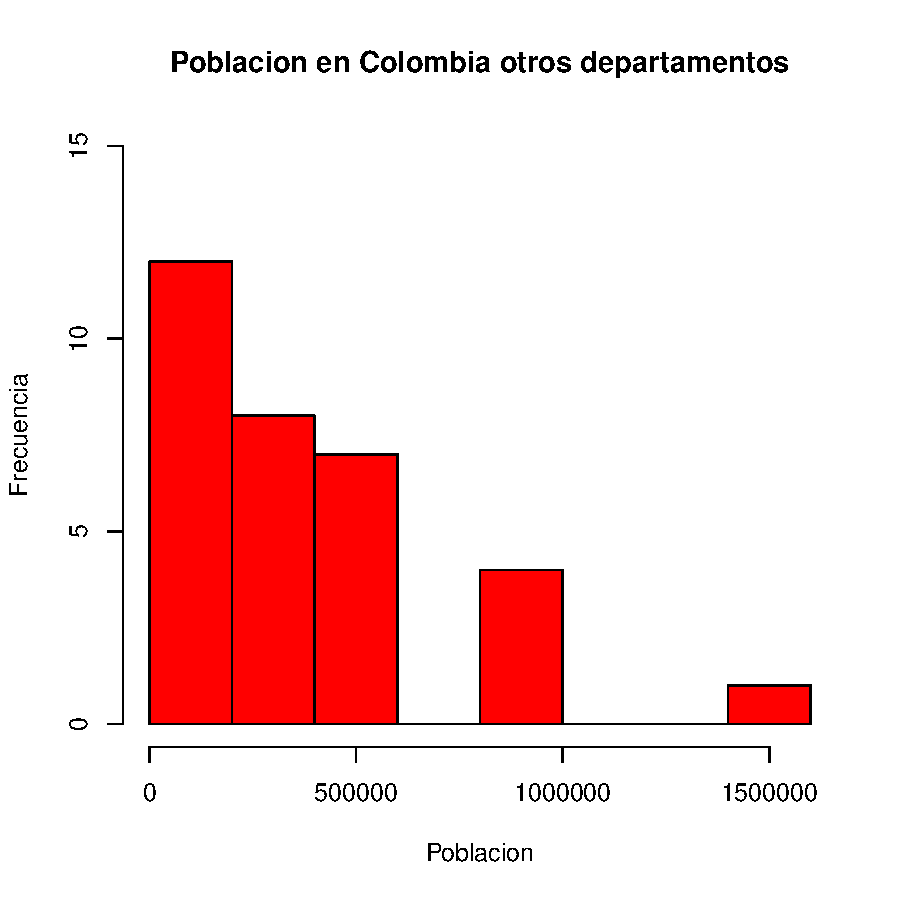
\includegraphics{univariada-summaryDatos}
\caption{Histograma de la poblacion en Colombia para los otros departamentos}
\label{barplot3}
\end{figure}
Los histogramas de los datos del indice se muestran en las figuras 
\begin{figure}[h]
\centering

dado el sesgo de las poblaciones, se realiza una transformaci�n de tal manera que se acerque a la realidad. En la figura \ref{barplot4} se muestra el resultado de esta transformaci\'on.

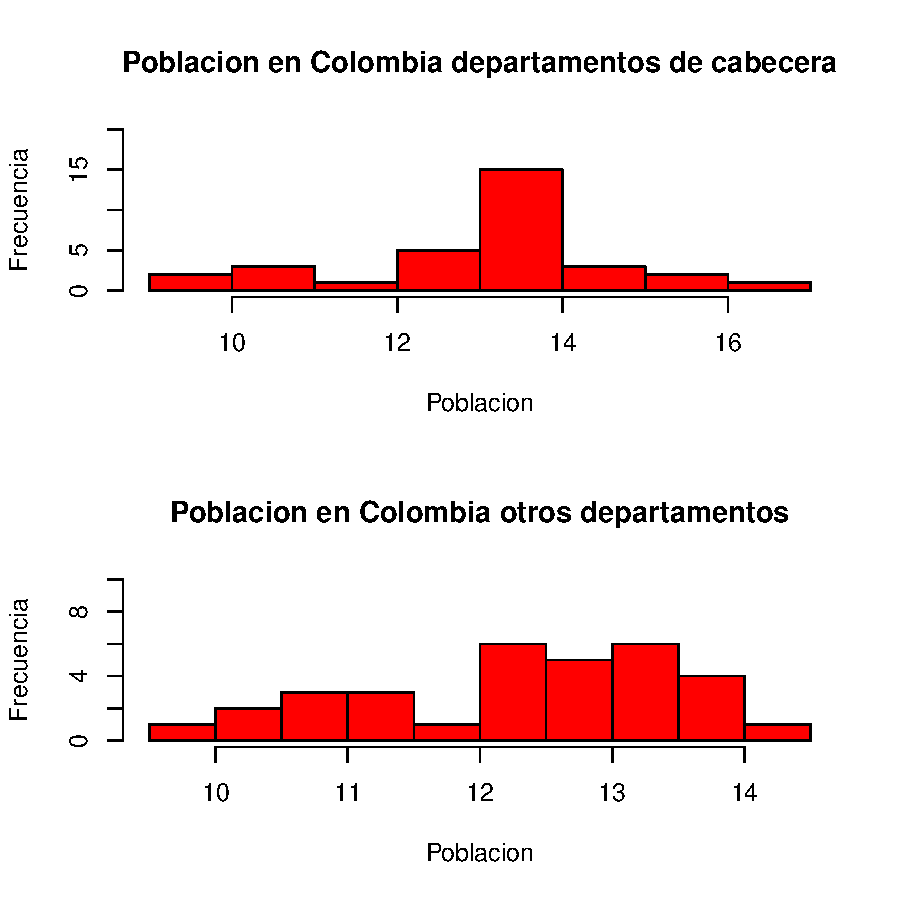
\includegraphics{univariada-rehacerhistogramas}
\caption{Histograma transformado de la poblacion en Colombia para los 32 departamentos}
\label{barplot4}
\end{figure}
